\documentclass[a4paper,10pt]{article}
\usepackage[polish]{babel}
\usepackage[utf8]{inputenc}
\usepackage[T1]{fontenc}
\usepackage{times}
\usepackage{graphicx}
\usepackage{anysize}

%\marginsize{left}{right}{top}{bottom}
\marginsize{2.5cm}{2.5cm}{2.5cm}{2.5cm}


\begin{document}
\section{Wprowadzenie}
\label{sec:wprowadzenie}

Nauka zajmująca się badaniem i~poznawaniem budowy organizmów ptaków oraz ich życia nosi nazwę \emph{ornitologii} i~jest częścią \emph{zoologii}. Do tej dyscypliny naukowej należy morfologia, tj. nauka o~wyglądzie i~budowie zewnętrznej i~wewnętrznej ptaka, biologia -- nauka o~wszelkich przejawach ich życia fizycznego: ekologia, nauka o~wymaganych przez dany gatunek warunkach środowiskowych oraz etologia -- nauka o~zwyczajach i~sposobie zachowania się poszczególnych gatunków. W~zakres wiedzy ornitologicznej wchodzi również systematyka zoologiczna, polegająca na podziale wszystkich ptaków na grupy systematyczne (gromada, rząd, rodzina, rodzaj, gatunek) według bliższego lub dalszego pokrewieństwa. 

Niezależnie od systematyki przyjęto tutaj podział wszystkich ptaków na trzy grupy według ich użyteczności gospodarczej: ptaki łowne, które w~okresie lęgów znajdują się pod tzw. ochroną okresową, ptaki objęte całoroczną ochroną, zwaną gatunkową, ptaki, które w~ciągu całego roku w~ogóle nie podlegają ochronie.

\medskip
\begin{minipage}{4cm}
	\centerline{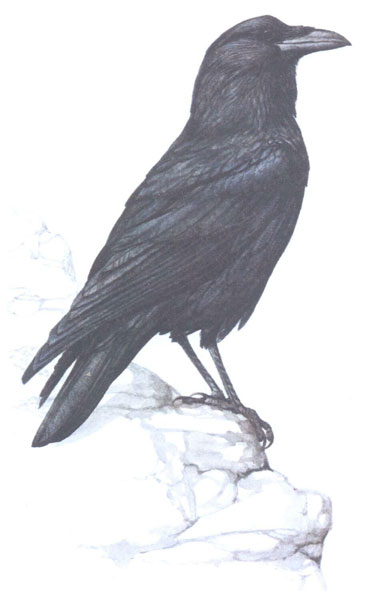
\includegraphics[scale=0.4]{kruk}}
\end{minipage}
\hspace{5mm}
\medskip
\begin{minipage}{11cm}
\section{Rodzina krukowatych}
\label{sec:rodzinakrukowatych}

\subsection{Kruk}

Stosunkowo nieliczny gatunek osiadły i~zalatujący. Żyje w~starych lasach, w~pobliżu których znajdują się skaliste zbocza, poręby, łąki, miejsca rzadko odwiedzane. Gatunek monogamiczny łączący się w~pary prawdopodobnie na całe życie. Okres gniazdowania: luty-kwiecień. Gniazda buduje z gałązek, umieszcza na drzewie lub na skale, samica wyściela je miękkim materiałem. Składa 4-6 zielonkawych jaj kształtu jajowatego z~brązowymi plamami. Wysiaduje wyłącznie samica przez około 3~tygodnie; samiec ją w~tym czasie żywi. Pisklęta są gniazdownikami, karmione przez obydwoje rodziców około 40 dni. 
\end{minipage}
\medskip
 \begin{minipage}{11cm}

\section{Rodzina jaskółkowatych}

\subsection{Jaskółka oknówka}

Liczny gatunek lęgowy i~przelotny. Przylatuje w~kwietniu, odlatuje we wrześniu. Przebywa w~miejscach, w~których żyje również jaskółka dymówka. Gniazdo buduje pod dachami budynków, rzadziej gnieździ się wewnątrz budynku. Gniazdo jest ulepione z~gliny zmieszanej z~błotem i~śliną, w~kształcie ćwierć kuli przyczepionej pod okapem dachu do ściany. Wewnątrz wysłane jest pierzem i~sierścią. Gatunek monogamiczny. Gniazduje dwa razy w~ciągu roku. Znosi 4-5 czystobiałych jaj, kształtu jajowatego. Wysiaduje samiczka i~samiec przez około dwa tygodnie. Pisklęta karmione przez 21-23 dni, są rzekomymi gniazdownikami, lęgną się okryte białawym puchem. Wykarmianie piskląt trwa około 24 dni.
\end{minipage}
\begin{minipage}{7cm}
	\centerline{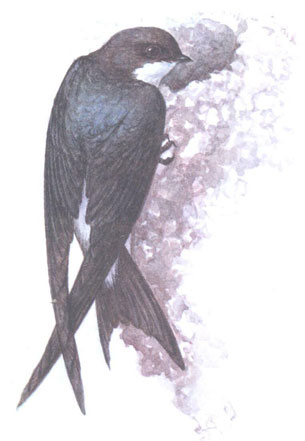
\includegraphics[scale=0.4]{jaskolka-oknowka}}
\end{minipage}

\end{document}
